\chapter{Quantum Computing Foundations}
\label{chap:quantum_foundations}

This chapter introduces the quantum computing concepts that underpin the machine learning models used in this work. I cover qubits, quantum gates, measurement, data encoding strategies, parameterized quantum circuits, and the constraints of current quantum hardware.

% ============================================================
\section{Qubits and Superposition}
\label{sec:qubits}

In classical computing, the fundamental unit of information is the bit, which takes a value of either 0 or~1. In quantum computing, the analogous unit is the \emph{qubit}~\cite{nielsen2010quantum}. A qubit is a two-level quantum system whose state is a vector in a two-dimensional complex Hilbert space. The two basis states are denoted $\ket{0}$ and $\ket{1}$, and a qubit can exist in a \emph{superposition} of both:
\begin{equation}
    \ket{\psi} = \alpha \ket{0} + \beta \ket{1}, \qquad |\alpha|^2 + |\beta|^2 = 1,
    \label{eq:superposition}
\end{equation}
where $\alpha, \beta \in \mathbb{C}$ are complex amplitudes. The values $|\alpha|^2$ and $|\beta|^2$ represent the probabilities of obtaining outcomes 0 and~1 upon measurement.

Since global phase is unobservable, any single-qubit state can be parameterized by two angles $\theta \in [0, \pi]$ and $\varphi \in [0, 2\pi)$:
\begin{equation}
    \ket{\psi} = \cos\frac{\theta}{2}\,\ket{0} + e^{i\varphi}\sin\frac{\theta}{2}\,\ket{1}.
    \label{eq:bloch}
\end{equation}

This defines a point on the \emph{Bloch sphere} (Figure~\ref{fig:bloch_sphere}), a unit sphere in $\mathbb{R}^3$ where $\ket{0}$ is the north pole, $\ket{1}$ the south pole, and every quantum gate corresponds to a rotation of this sphere.

\begin{figure}[ht]
    \centering
    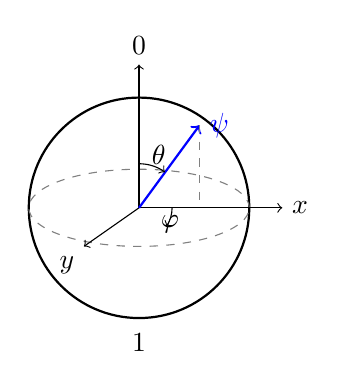
\begin{tikzpicture}[scale=1.4]
        \draw[thick] (0,0) circle (1);
        \draw[dashed, gray] (0,0) ellipse (1 and 0.35);
        \draw[->] (0,0) -- (1.3,0) node[right] {$x$};
        \draw[->] (0,0) -- (0,1.3) node[above] {$\ket{0}$};
        \draw[->] (0,0) -- (-0.5,-0.35) node[below left] {$y$};
        \node[below] at (0,-1.05) {$\ket{1}$};
        \draw[->, thick, blue] (0,0) -- (0.55, 0.75) node[right] {$\ket{\psi}$};
        \draw[dashed, gray] (0.55, 0.75) -- (0.55, 0);
        \draw[->] (0, 0.4) arc (90:54:0.4);
        \node at (0.18, 0.48) {$\theta$};
        \draw[->] (0.3, 0) arc (0:-35:0.3);
        \node at (0.28, -0.15) {$\varphi$};
    \end{tikzpicture}
    \caption{The Bloch sphere. Any pure single-qubit state $\ket{\psi}$ corresponds to a point on the surface, parameterized by angles $\theta$ and $\varphi$.}
    \label{fig:bloch_sphere}
\end{figure}
% ============================================================
\section{Multi-Qubit Systems and Entanglement}
\label{sec:multiqubit}
The joint state space of $n$~qubits is a $2^n$-dimensional Hilbert space. A general pure state can be written as
\[
\ket{\Psi} = \sum_{j=0}^{2^n-1} c_j \ket{j},
\qquad
\sum_{j=0}^{2^n-1} |c_j|^2 = 1,
\]
where $c_j \in \mathbb{C}$ are complex amplitudes and $\{\ket{j}\}$ denotes the computational basis states.

A state is said to be \emph{entangled} if it cannot be factorized as a tensor product of individual qubit states. A canonical example is the Bell state:
\begin{equation}
    \ket{\Phi^+} = \frac{1}{\sqrt{2}} \big( \ket{00} + \ket{11} \big),
\end{equation}
whose measurement outcomes are perfectly correlated: measuring one qubit determines the outcome of the other.

Entanglement plays a central role in quantum machine learning. Entangling gates applied between qubits encoding different input features allow the circuit to capture correlations that would otherwise require significantly more parameters in a classical model~\cite{hur2022quantum}.
% ============================================================


\section{Quantum Gates}
\label{sec:gates}

Quantum gates are unitary transformations that manipulate qubit states. For quantum machine learning, the most important gates are built from the \emph{Pauli matrices} and the Hadamard gate.

\subsection{Pauli Matrices}

The three Pauli matrices form a basis for all single-qubit operations and play a central role throughout quantum computing:
\begin{equation}
    X = \begin{pmatrix} 0 & 1 \\ 1 & 0 \end{pmatrix}, \quad
    Y = \begin{pmatrix} 0 & -i \\ i & 0 \end{pmatrix}, \quad
    Z = \begin{pmatrix} 1 & 0 \\ 0 & -1 \end{pmatrix}.
    \label{eq:pauli}
\end{equation}

Each Pauli matrix is Hermitian and unitary, with $P^2 = I$. In this work they play two direct roles: the rotation gates $R_x(\theta)$, $R_y(\theta)$, $R_z(\theta)$ used as trainable gates throughout are defined as their matrix exponentials (Equation~\ref{eq:rotations}); and the Pauli-$Z$ matrix serves as the measurement observable whose expectation value $\langle Z \rangle$ is the output of every classifier in this work.

\subsection{Rotation Gates}

The parameterized rotation gates rotate the Bloch vector around the $x$, $y$, or $z$ axis by an angle~$\theta$:
\begin{equation}
    R_x(\theta) = e^{-i\frac{\theta}{2}X}, \qquad
    R_y(\theta) = e^{-i\frac{\theta}{2}Y}, \qquad
    R_z(\theta) = e^{-i\frac{\theta}{2}Z}.
    \label{eq:rotations}
\end{equation}

Any single-qubit unitary can be decomposed as $U = R_z(\alpha)\,R_y(\beta)\,R_z(\gamma)$ up to global phase~\cite{nielsen2010quantum}. In quantum machine learning, the angles are either set by the input data (encoding) or treated as trainable parameters (optimization).

\subsection{Hadamard and Entangling Gates}

The \textbf{Hadamard gate} $H = \frac{1}{\sqrt{2}}\big(X + Z\big)$ maps $\ket{0}$ to the equal superposition $\frac{1}{\sqrt{2}}(\ket{0}+\ket{1})$ and is used to initialize qubits in superposition.

For multi-qubit circuits, \textbf{entangling gates} create correlations between qubits. The \emph{CNOT} gate flips the target qubit when the control is $\ket{1}$. The \emph{CZ} gate applies a phase flip $\ket{11} \to -\ket{11}$. Both are used in variational circuits to build correlations between encoded features~\cite{cerezo2021variational}.
% ============================================================
\section{Measurement}
\label{sec:measurement}

Measurement extracts classical information from a quantum state. Measuring $\ket{\Psi} = \sum_j c_j \ket{j}$ in the computational basis yields outcome~$j$ with probability $P(j) = |c_j|^2$ (the \emph{Born rule}), after which the state collapses to $\ket{j}$.

In quantum machine learning, the circuit output is typically an \emph{expectation value} of an observable, most commonly the Pauli-$Z$ operator on an output qubit:
\begin{equation}
    \langle Z \rangle = P(0) - P(1) \;\in\; [-1,\, 1].
    \label{eq:expectation}
\end{equation}
This value serves as the raw prediction of the quantum classifier. Since measurement is probabilistic, the circuit must be executed multiple times (\emph{shots}) to estimate $\langle Z \rangle$ with sufficient precision.
% ============================================================

\section{Data Encoding}
\label{sec:encoding}

A critical step in quantum machine learning is \emph{data encoding} (also called \emph{feature mapping}): the process of embedding classical data $\mathbf{x} \in \mathbb{R}^d$ into a quantum state. The choice of encoding determines how many qubits are required, the circuit depth, and fundamentally shapes what functions the quantum model can learn~\cite{larose2020robust, schuld2021effect}. Three principal methods exist.

\subsection{Angle Encoding}

In angle encoding, each feature $x_i$ is mapped to a rotation angle on a dedicated qubit~\cite{schuld2020circuit}:
\begin{equation}
    S(\mathbf{x}) = \bigotimes_{i=1}^{d} R_y(x_i)\ket{0}.
    \label{eq:angle_encoding}
\end{equation}
This requires $d$~qubits (one per feature) but only a single layer of parallel rotations, giving a constant circuit depth of~1. It is the simplest and most widely used method. Its main limitation is that the number of qubits scales linearly with the number of features, so dimensionality reduction must be applied for high-dimensional datasets.

\subsection{Dense Encoding (Data Re-uploading)}

Dense encoding, introduced by P\'erez-Salinas et al.~\cite{perez2020data}, takes a fundamentally different approach: instead of dedicating one qubit per feature, it encodes \emph{multiple features into a single qubit} by applying successive parameterized rotations across multiple layers. The data is \emph{re-uploaded} at each layer, interleaved with trainable parameters. This method uses very few qubits but requires circuit depth proportional to the number of layers $L$ (detailed in Chapter~\ref{chap:architectures}).

Table~\ref{tab:encoding} summarizes the trade-offs between the two methods used in this work.

\begin{table}[ht]
    \centering
    \begin{tabular}{lccc}
        \toprule
        \textbf{Method} & \textbf{Qubits} & \textbf{Depth} & \textbf{Features/qubit} \\
        \midrule
        Angle encoding       & $d$ & $\mathcal{O}(1)$ & 1 \\
        Dense (re-uploading) & 1   & $\mathcal{O}(L)$ & all per layer \\
        \bottomrule
    \end{tabular}
    \caption{Comparison of data encoding methods. $d$: number of features, $L$: number of re-uploading layers.}
    \label{tab:encoding}
\end{table}

In this work, I use angle encoding for the QCNN and dense encoding for the data re-uploading classifier.

% ============================================================
\section{Parameterized Quantum Circuits and Training}
\label{sec:pqc}

A \emph{parameterized quantum circuit} (PQC) is the quantum analogue of a neural network~\cite{benedetti2019parameterized}. It consists of three stages: (1)~data encoding, (2)~a sequence of trainable rotation gates interleaved with entangling gates, and (3)~measurement. The output defines a function 
\[
f(\mathbf{x}; \boldsymbol{\theta}) = \bra{0^n} U^\dagger(\mathbf{x}, \boldsymbol{\theta})\, Z\, U(\mathbf{x}, \boldsymbol{\theta}) \ket{0^n},
\]
where $\boldsymbol{\theta}$ are the trainable parameters.

To optimize $\boldsymbol{\theta}$, gradients are computed using the \emph{parameter-shift rule}~\cite{mitarai2018quantum}: for each parameter $\theta_k$ appearing in a rotation gate, the partial derivative is:
\begin{equation}
    \frac{\partial f}{\partial \theta_k} 
    = \frac{1}{2}\Big[ 
    f\!\big(\theta_k + \tfrac{\pi}{2}\big) 
    - 
    f\!\big(\theta_k - \tfrac{\pi}{2}\big) 
    \Big].
    \label{eq:param_shift}
\end{equation}

This provides exact gradients without finite-difference approximations; PennyLane~\cite{pennylane} implements it automatically.
% ============================================================
\section{NISQ Constraints}
\label{sec:nisq}

Current quantum computers are Noisy Intermediate-Scale Quantum (NISQ) devices~\cite{preskill2018quantum}, characterized by three limitations: (1)~a small number of qubits (tens to hundreds), limiting the data dimensionality that can be directly encoded; (2)~gate errors and \emph{decoherence}, which impose an upper bound on circuit depth before outputs become unreliable; and (3)~limited qubit connectivity, requiring extra SWAP gates for non-adjacent interactions.

These constraints motivate shallow-depth architectures. The data re-uploading approach~\cite{perez2020data} achieves universality with linear depth using only one or a few qubits. The QCNN~\cite{hur2022quantum} achieves logarithmic depth through hierarchical pooling and has been shown to avoid the \emph{barren plateau} problem~\cite{mcclean2018barren}, where gradients vanish exponentially with circuit size.

In this work, all experiments use noiseless simulation via PennyLane, but the circuit designs are chosen to be compatible with near-term hardware: shallow depth, nearest-neighbor connectivity, and a small number of qubits.

